\documentclass[11pt,a4paper,oneside]{report}


\usepackage{amsmath,amssymb,calc,ifthen}

\usepackage{float}

\usepackage[table,usenames,dvipsnames]{xcolor} % for coloured cells in tables

\usepackage{tikz}

% Allows us to click on links and references!

\usepackage{hyperref}
\hypersetup{
    colorlinks,
    citecolor=black,
    filecolor=black,
    linkcolor=black,
    urlcolor=black
}

% Nice package for plotting graphs
% See excellent guide:
% http://www.tug.org/TUGboat/tb31-1/tb97wright-pgfplots.pdf
\usetikzlibrary{plotmarks}
\usepackage{amsmath,graphicx}
\usepackage{epstopdf}
\usepackage{caption}
\usepackage{subcaption}

% highlight - useful for TODOs and similar
\usepackage{color}
\newcommand{\hilight}[1]{\colorbox{yellow}{#1}}

\newcommand\ci{\perp\!\!\!\perp} % perpendicular sign
\newcommand*\rfrac[2]{{}^{#1}\!/_{#2}} % diagonal fraction

\usepackage{listings}



% margin size
\usepackage[margin=1in]{geometry}

\tikzstyle{state}=[circle,thick,draw=black, align=center, minimum size=2.1cm,
inner sep=0]
\tikzstyle{vertex}=[circle,thick,draw=black]
\tikzstyle{terminal}=[rectangle,thick,draw=black]
\tikzstyle{edge} = [draw,thick]
\tikzstyle{lo} = [edge,dotted]
\tikzstyle{hi} = [edge]
\tikzstyle{trans} = [edge,->]


\definecolor{mygreen}{rgb}{0,0.6,0}
\definecolor{mygray}{rgb}{0.5,0.5,0.5}
\definecolor{mymauve}{rgb}{0.58,0,0.82}

\lstset{ %
  backgroundcolor=\color{white},   % choose the background color; you must add 
%\usepackage{color} or \usepackage{xcolor}
  basicstyle=\footnotesize,        % the size of the fonts that are used for the 
%code
  breakatwhitespace=false,         % sets if automatic breaks should only happen 
%at whitespace
  breaklines=true,                 % sets automatic line breaking
  captionpos=b,                    % sets the caption-position to bottom
  commentstyle=\color{mygreen},    % comment style
  deletekeywords={...},            % if you want to delete keywords from the 
%given language
  escapeinside={\%*}{*)},          % if you want to add LaTeX within your code
  extendedchars=true,              % lets you use non-ASCII characters; for 
%8-bits encodings only, does not work with UTF-8
  frame=single,                    % adds a frame around the code
  keepspaces=true,                 % keeps spaces in text, useful for keeping 
%indentation of code (possibly needs columns=flexible)
  keywordstyle=\color{blue},       % keyword style
  language=Octave,                 % the language of the code
  morekeywords={*,...},            % if you want to add more keywords to the set
  numbers=left,                    % where to put the line-numbers; possible 
%values are (none, left, right)
  numbersep=5pt,                   % how far the line-numbers are from the code
  numberstyle=\tiny\color{mygray}, % the style that is used for the line-numbers
  rulecolor=\color{black},         % if not set, the frame-color may be changed 
%on line-breaks within not-black text (e.g. comments (green here))
  showspaces=false,                % show spaces everywhere adding particular 
%underscores; it overrides 'showstringspaces'
  showstringspaces=false,          % underline spaces within strings only
  showtabs=false,                  % show tabs within strings adding particular 
%underscores
  stepnumber=2,                    % the step between two line-numbers. If it's 
%1, each line will be numbered
  stringstyle=\color{mymauve},     % string literal style
  tabsize=2,                       % sets default tabsize to 2 spaces
  title=\lstname                   % show the filename of files included with 
%\lstinputlisting; also try caption instead of title
}


\title{Graphical Models Coursework 1}
\author{
    Razvan Valentin Marinescu\\
    \texttt{razvan.marinescu.14@ucl.ac.uk}
    \and
    David Owen\\
    \texttt{email.address@ucl.ac.uk}
    \and
    Kin Quan\\
    \texttt{email.address@ucl.ac.uk}
}

\begin{document}
\belowdisplayskip=12pt plus 3pt minus 9pt
\belowdisplayshortskip=7pt plus 3pt minus 4pt

\maketitle{}


\section*{Problem 2.5}
Hello

\section*{Problem 2.6}


\section*{Problem 2.7}


\section*{Problem 2.9}


\section*{Problem 3.3}

\begin{itemize}
 \item $tuberculosis \ci smoking\;|\; shortness\;of\;breath$ is \textbf{false}, 
because path $t \to e \to d \to b \to s$ is not blocked
 \item $lung\;cancer \ci  bronchitis\;|\;smoking$ is \textbf{true}, because:
  \begin{itemize}
    \item path $l \to s \to b$ is blocked ($s$ is instantiated)
    \item path $l \to e \to d \to b$ is blocked (has collider ${e,d,b}$)
  \end{itemize}
 \item $visit \; to \; Asia \ci smoking\;|\;lung\;cancer$ is \textbf{true}, 
because:
   \begin{itemize}
    \item path $a \to t \to e \to l \to s$ is blocked ($l$ is instantiated)
    \item path $a \to t \to e \to d \to b \to s$ is blocked ($d$ is 
uninstantiated)
  \end{itemize}
 \item $visit \; to \; Asia \ci smoking\;|\;lung \; cancer; \; shortness \; of 
\; breath$ is \textbf{false} because path $a \to t \to e \to d \to b \to s$ is 
not blocked ($d$ is instantiated).
\end{itemize}



\section*{Problem 3.4}


\section*{Problem 3.8}


\section*{Problem 3.9}

\subsection*{1. Belief network}

\begin{figure}[H]
  \centering
    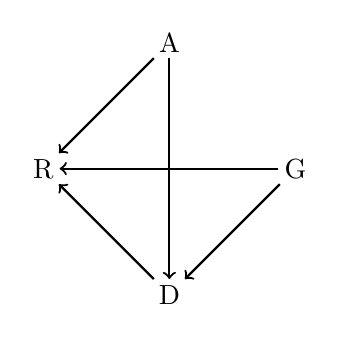
\begin{tikzpicture}[scale=0.8,help lines/.style={color=lightgray,line 
width=0.2pt},post/.style={->,shorten >=1pt,>=stealth',thick}]
    
    \node[inner sep=2] (A) at (0.0,2.0){A};
    \node[inner sep=2] (G) at (2.0,0.0) {G};
    \node[inner sep=2] (R) at (-2.0,0.0) {R};
    \node[inner sep=2] (D) at (0.0,-2.0) {D};

    \draw[->, thick] (A) -- (R);
    \draw[->, thick] (A) -- (D);
    \draw[->, thick] (G) -- (D);
    \draw[->, thick] (G) -- (R);
    \draw[->, thick] (D) -- (R);
    
    \end{tikzpicture}
    \caption{Belief network}
    \label{fig:all_trade_cca_black}     
\end{figure}

\subsection*{2. Computation of $p(recover \; | \; drug)$}

Applying Bayes rule we get $p(recover \; | \; drug) = \frac{p(recover, 
\;drug)}{p(drug)}$. This suggests that from a database of patient entries we 
take the number of patients that both recovered and received the drug and 
divide 
it by the number of patients that received the drug. 

\subsection*{3. Computation of $p(recover \; | \; do(drug),\; yound)$}

\hilight{David, could you please write the answer for this one?}

\section*{Problem 3.11}


\section*{Problem 3.12}


\section*{Problem 3.13}


\section*{Problem 3.14}


\section*{Problem 3.15}


\section*{Problem 3.17}

\subsection*{1.}

In order to prove $a \ci c$ we need to show that $p(a,c) = p(a)p(c)$. We first 
calculate the joint probability distribution $p(a,b,c) = p(c|b)p(b|a)p(a)$. 
Then 
we marginalise over $b$ to get $p(a,c)=\sum_{b} p(a,b,c) = \sum_{b} 
p(c|b)p(b|a)p(a)$. 

We will now calculate the three terms from the sum $\sum_{b} 
p(c|b)p(b|a)p(a)$. For $b=1$ we get 

% b = 1

\begin{equation}
\label{317A}
p(b = 1|a) =  
  \begin{pmatrix}
   \ 1/4 \\[0.4em]
   \ 15/40 \\
 \end{pmatrix}
\end{equation}

 
\begin{equation}
\label{317B}
    p(b = 1, a) = p(b = 1|a) p(a) = \begin{pmatrix}
      \ 3/20 \\[0.4em]
      \ 3/20 \\
    \end{pmatrix}
\end{equation}

\begin{equation}
\label{317C}
p(c | b = 1) =  
  \begin{pmatrix}
   \ 1/3 \\[0.4em]
   \ 2/3 \\
 \end{pmatrix} 
\end{equation}

Combining equations \eqref{317B} and \eqref{317C} we get:

\begin{equation}
\label{317D}
p(a, b = 1, c) =  p(c | b = 1 )p(b = 1,a)
  \begin{pmatrix}
   \ \frac{3}{20} \frac{1}{3} & \frac{3}{20} \frac{2}{3} \\[0.4em]
   \ \frac{3}{20} \frac{1}{3} & \frac{3}{20} \frac{2}{3} \\
 \end{pmatrix} = \frac{1}{40}
  \begin{pmatrix}
   \ 2 & 4 \\[0.4em]
   \ 2 & 4 \\
 \end{pmatrix} 
\end{equation}

A similar computaiton is done for $p(a, b = 2, c)$ and $p(a, b = 3, c)$. 

% b =2

\begin{equation}
\label{317E}
    p(b = 2, a) = p(b = 2|a) p(a) = 
    \begin{pmatrix}
      \ \frac{1}{12} \frac{3}{5} \\[0.4em]
      \ \frac{1}{8} \frac{2}{5} \\
    \end{pmatrix} = 
    \begin{pmatrix}
      \ 1/20 \\[0.4em]
      \ 1/20 \\
    \end{pmatrix}
\end{equation}

\begin{equation}
\label{317F}
p(c | b = 2) =  
  \begin{pmatrix}
   \ 1/2 \\[0.4em]
   \ 1/2 \\
 \end{pmatrix} 
\end{equation}

Combining equations \eqref{317E} and \eqref{317F} we get:

\begin{equation}
\label{317G}
p(a, b = 2, c) =  
  \begin{pmatrix}
   \ \frac{1}{20} \frac{1}{2} & \frac{1}{20} \frac{1}{2} \\[0.4em]
   \ \frac{1}{20} \frac{1}{2} & \frac{1}{20} \frac{1}{2} \\
 \end{pmatrix} = \frac{1}{40}
  \begin{pmatrix}
   \ 1 & 1 \\[0.4em]
   \ 1 & 1 \\
 \end{pmatrix} 
\end{equation}

%% b = 3

Now for $b = 3$ we get:

\begin{equation}
\label{317H}
    p(b = 3, a) = p(b = 3|a) p(a) = 
    \begin{pmatrix}
      \ \frac{2}{3} \frac{3}{5} \\[0.4em]
      \ \frac{1}{2} \frac{2}{5} \\
    \end{pmatrix} = \frac{1}{5}
    \begin{pmatrix}
      \ 2 \\[0.4em]
      \ 1 \\
    \end{pmatrix}
\end{equation}

\begin{equation}
\label{317I}
p(c | b = 3) =  
  \begin{pmatrix}
   \ 15/40 \\[0.4em]
   \ 5/8 \\
 \end{pmatrix} 
\end{equation}

Combining equations \eqref{317H} and \eqref{317I} we get:

\begin{equation}
\label{317J}
p(a, b = 3, c) =  
  \begin{pmatrix}
   \ \frac{2}{5} \frac{15}{40} & \frac{2}{5} \frac{5}{8} \\[0.4em]
   \ \frac{1}{5} \frac{15}{40} & \frac{1}{5} \frac{5}{8} \\
 \end{pmatrix} = \frac{1}{40}
  \begin{pmatrix}
   \ 6 & 10 \\[0.4em]
   \ 3 & 5 \\
 \end{pmatrix} 
\end{equation}

Summing up all the right-hand side terms from equations \eqref{317D},  
\eqref{317G} and  \eqref{317J} we get

\begin{equation}
\label{317K}
p(a, c) =  \sum_{b} p(a,b,c) = \frac{1}{40}
  \begin{pmatrix}
   \ 9 & 15 \\[0.4em]
   \ 6 & 10 \\
 \end{pmatrix} 
\end{equation}
 
From the joint distribution $p(a,c)$ we can calculate the marginalise

\begin{equation}
\label{317L}
p(c) =  \sum_{a} p(a,c) = \frac{1}{8}
  \begin{pmatrix}
   \ 3 \\[0.4em]
   \ 5 \\
 \end{pmatrix} 
\end{equation}
 
Using the given distribution $p(a)$ and the above equation we can now calculate:
\begin{equation}
\label{317M}
p(a)p(c) =
  \begin{pmatrix}
   \ \frac{3}{5} \frac{3}{8} & \frac{3}{5} \frac{5}{8} \\[0.4em]
   \ \frac{2}{5} \frac{3}{8} & \frac{2}{5} \frac{5}{8} \\
 \end{pmatrix} = \frac{1}{40}
  \begin{pmatrix}
   \ 9 & 15 \\[0.4em]
   \ 6 & 10 \\
 \end{pmatrix} 
\end{equation}

From equations \eqref{317K} and \eqref{317M} it results that $p(a,c) = p(a)p(c)$ 
which implies $a \ci c$

\subsection*{2.}

We are given that:

\begin{equation}
\label{317N}
p(a,b,c) = \frac{1}{Z}\phi(a, b)\psi(b,c). 
\end{equation}
Looking at the element at position $(i,j)$ in the $MN^\top$ matrix we notice 
that:
\begin{equation}
\frac{1}{Z}\left[ MN^\top \right]_{ik} = \frac{1}{Z}\sum_{j}\phi(a=i, 
b=j)\psi(b=j, c=k). 
\end{equation}
Applying equation \eqref{317N} in the right hand side term above we get:
\begin{equation}
\frac{1}{Z}\sum_{j}\phi(a=i, b=j)\psi(b=j, c=k) = \sum_{j}p(a = i, b = j, c = k) 
= p(a = i, c = k) 
\end{equation}
which implies that
\begin{equation}
\frac{1}{Z}\left[ MN^\top \right]_{ik} = p(a = i, c = k) 
\end{equation}

\subsection*{3.}

Using the given and the result from the previous subpoint we get
\begin{equation}
 \frac{1}{Z}\left[ MN^\top \right] = m_0n_0^\top = p(a, c) 
\end{equation}
and $\forall i,j$
\begin{equation}
 m_0(i)n_0(j) = p(a=i, c=j) 
\end{equation}
If we define functions $f(i)=m_0(i)$ and $g(j)=n_0(j)$, $\forall i \in dom(a), j 
\in dom(c)$ then we get:
$$ p(a,c) = \frac{1}{Z}f(a)g(c)$$ which implies $a \ci c$

\subsection*{4.}

$\forall (i,j) \in dim(MN^\top)$ we have:
$$MN^\top(i,j) = \sum_{k=1}^{3}M(i,k)N^\top(k,j) = \sum_{k=1}^{3} m_k(i)n_k(j) = 
m_1n_1^\top(i,j) + m_2n_2^\top(i,j) + m_3n_3^\top(i,j)$$  
which implies that:
$$ MN^\top = m_1n_1^\top + m_2n_2^\top + m_3n_3^\top$$

\subsection*{5.}

From the previous results and from the definitions of $m_2$ and $n_3$ we get:
$$MN^\top = m_1n_1^\top + m_2n_2^\top + m_3n_3^\top = m_1n_1^\top + \lambda 
m_1n_2^\top + m_3\gamma(n_1^\top + \lambda n_2^\top)$$
Factorising further we get
$$MN^\top = m_1(n_1^\top + \lambda n_2^\top) + m_3\gamma (n_1^\top + \lambda 
n_2^\top) = (m_1 + \gamma m_3)(n_1^\top + \lambda n_2^\top) = m_0n_0^\top$$

\subsection*{6.}

Let us set $\lambda = 1$ and $\gamma = 1$ and the following vectors:

$m_1 =   
 \begin{pmatrix}
   \ 2  \\[0.4em]
   \ 1  \\
 \end{pmatrix} 
$  
$m_2 =   
 \begin{pmatrix}
   \ 2  \\[0.4em]
   \ 1  \\
 \end{pmatrix} 
$  
$m_3 =   
 \begin{pmatrix}
   \ 0  \\[0.4em]
   \ 3  \\
 \end{pmatrix} 
$  
$n_1 =   
 \begin{pmatrix}
   \ 2  \\[0.4em]
   \ 2  \\
 \end{pmatrix} 
$  
$n_2 =   
 \begin{pmatrix}
   \ 1  \\[0.4em]
   \ 3  \\
 \end{pmatrix} 
$  
$n_3 =   
 \begin{pmatrix}
   \ 3  \\[0.4em]
   \ 5  \\
 \end{pmatrix}
 $\\\\
This gives us the following matrices:

$ M = 
 \begin{pmatrix}
   \ 2 & 1 \\[0.4em]
   \ 2 & 1 \\[0.4em]
   \ 0 & 3
 \end{pmatrix}
$
$ N^\top = 
 \begin{pmatrix}
   \ 2 & 1 & 3 \\[0.4em]
   \ 2 & 3 & 5
 \end{pmatrix}
$\\\\
Setting $p(a) = 
 \begin{pmatrix}
   \ 1/2 \\[0.4em]
   \ 1/2
 \end{pmatrix}
$ gives the following conditional tables:

$ p(b|a) = \begin{pmatrix}
   \ 1/2 & 1/5 \\[0.4em]
   \ 1/2 & 1/5 \\[0.4em]
   \ 0 & 3/5
 \end{pmatrix} 
$
$ p(c|b) = \begin{pmatrix}
   \ 1/2 & 1/4 & 3/8 \\[0.4em]
   \ 1/2 & 3/4 & 5/8
 \end{pmatrix} 
$

Running the following code in Julia (using the BRML toolbox) shows that $p(a,c) 
= p(a)p(c)$ which implies $a \ci c$. The code was adapted from 
\texttt{demoChainIndepRational.jl}

\begin{lstlisting}
A,B,C=1,2,3

pA = PotArray(A, [1//2, 1//2])

pBgA = PotArray([B A], [1//2 1//5; 1//2 1//5; 0 3//5])

pCgB = PotArray([C B], [1//2 1//4 3//8; 1//2 3//4 5//8])

pABC = pCgB * pBgA * pA
pAC = sum(pABC, B)

pA=sum(pAC,C)
pC=sum(pAC,A)

println("pAC-pA*pC=")
println(pAC-pA*pC)

\end{lstlisting}


\section*{Problem 3.20}


\section*{Problem 3.21}


\section*{Problem 3.22}


\section*{Extra Problem A}


\section*{Extra Problem B}


\end{document}
